% inspiration by Overleaf template (tikz)
% modified Truong Nhan Nguyen

\documentclass[tikz, border=10pt]{standalone}

\usepackage{tikz}
\usetikzlibrary{arrows, decorations.markings, backgrounds}
\usepackage{amsmath, amsfonts, amssymb, mathtools}

\tikzset{
    path/.style = {
        postaction={decorate,
            decoration={
                markings,
                mark=at position 1cm with {\arrow[]{stealth}}
            }
        }
    },
    force/.style = {-latex, ultra thick, cyan},
    vector/.style = {-latex, thick}
}

\begin{document}
    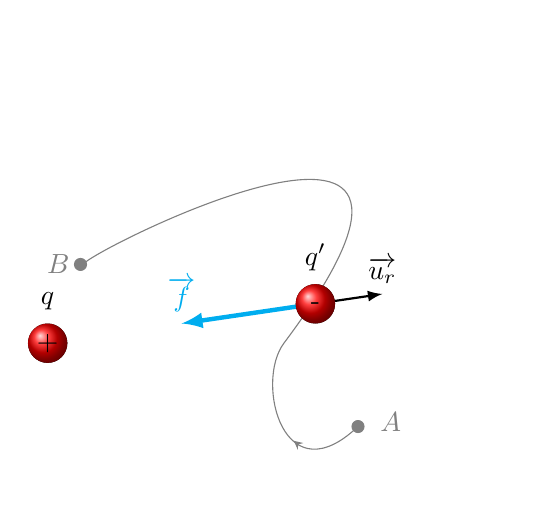
\begin{tikzpicture}
        \fill[ball color=red] (0, 0) circle (0.25) node{+}node[above=0.3cm] {$q$};
        \draw[path, *-*, color=gray] (4, -1) node[right=1mm] {$A$} ..controls+(-1, -1) and +(-0.375, -0.5).. (3, 0) .. controls +(3, 4) and (0.2, 1).. (0.5, 1) node[left=1mm] {$B$};
        \draw[force] (3.4, 0.5) -- ++(-1.7, -.25) node[above] {$\overrightarrow{f}$};
        \draw[vector] (3.4, 0.5) -- ++(.85, .125) node[above] {$\overrightarrow{u_r}$};
        \fill[ball color=red] (3.4, 0.5) circle (0.25) node{-}node[above=0.3cm] {$q^\prime$};
    \end{tikzpicture}
\end{document}